\chapter{DCM for Phase Coupling \label{Chap:data:dcm_phase}}

This chapter presents an extension of the Dynamic Causal Modelling (DCM) framework to the analysis of phase-coupled data. A weakly coupled oscillator approach is used to describe dynamic phase changes in a network of oscillators.
The influence that the phase of one oscillator has on the change of phase of another is characterised in terms of a Phase Interaction Function (PIF) as described in \cite{dcm_phase}. SPM supports PIFs specified using arbitrary order Fourier series. However, to simplify the interface, one is restricted to simple sinusoidal PIFs with the GUI. 

\section{Data}

We will use the merged epoched MEG dataset from Chapter~\ref{multimodal:data:meg}:

\begin{verbatim}
cdbespm8_SPM_CTF_MEG_example_faces1_3D.mat
cdbespm8_SPM_CTF_MEG_example_faces1_3D.dat
\end{verbatim}

See ~\ref{multimodal:data:meg:preproc} for instructions on how to generate this file from raw MEG data. DCM-Phase requires a head model and coregistration. If you have been following the previous chapters of this tutorial, these should already be available in the dataset. Otherwise, you should perform the 'Prepare' and '3D Source reconstruction' steps described earlier in the chapter, with the latter 
comprising the MRI, Co-register, Forward and Save sub-steps (see ~\ref{multimodal:data:meg:recon_pow}).

\section{Getting Started}

You need to start SPM and toggle ``EEG'' as the modality (bottom-right of SPM main window), or start SPM with \texttt{spm eeg}. In order for this to work you need to ensure that the main SPM directory is on your \matlab\ path.
After calling \texttt{spm eeg}, you see SPM's graphical user interface, the top-left window. The button for calling the DCM-GUI is found in the second partition from the top, on the right hand side. When pressing the button, the GUI pops up (Figure~\ref{dcm-ir:fig:1}).

\section{Data and design}

 You should switch the DCM model type to ``PHASE'' which is the option for DCM-Phase. Press ``new data'' and select the data file \texttt{cdbespm8\_\-SPM\_\-CTF\_\-MEG\_\-example\_\-faces1\_\-3D.mat}. This is an epoched data file with multiple trials per condition.  On the right-hand side enter the trial indices
\begin{verbatim}
1 2
\end{verbatim} 
for the 'face' and 'scrambled' evoked responses (we will model both trial types).
 The box below this list allows for specifying experimental effects on connectivity. Enter 
\begin{verbatim}
1 0
\end{verbatim} 
in the first row of the box. This means that ``face'' trial types can have different connectivity parameters than ''scrambled'' trial types. If we now click somewhere outside the box, a default name will be assigned to this effect - ``effect1''. It will appear in the small text box next to the coefficients box. It is possible to change this name to something else e.g. ``face''. Now we can select the peristimulus time window we want to model. 
Set it to:
\begin{verbatim}
1 300
\end{verbatim} 
ms. Select \texttt{1} for ``detrend'', to  remove the mean from each data record.  The \texttt{sub-trials} option makes it possible to select just a subset of trials for the analysis (select 2 for every second trial, 3 - for every third etc.). This is useful because DCM-Phase takes quite a long time to invert for all the trials and you might want to first try a smaller subset to get an idea about the possible results. Here we will assume that you used all the trials (sub-trials was set to 1). You can now click on the $>$ (forward) button, which will bring you to the next stage \textit{electromagnetic model}. From this part, you can press the red $<$ button to get back to the data and design part.

\section{Electromagnetic model}

With DCM-Phase, there are two options for how to extract the source data. Firstly, you can use 3 orthogonal single equivalent current dipoles (ECD) for each source, invert the resulting source model to get 3 source waveforms and take the first principal component. This option is suitable for multichannel EEG or MEG data. Alternatively, you can treat each channel as a source (LFP option). This is appropriate when the channels already contain source data either recorded directly with intracranial electrodes or extracted (e.g. using a beamformer). 

Note that a difference to DCM for evoked responses is that the parameters of the spatial model are not optimized. This means that DCM-Phase (like DCM-IR) will project the data into source space using the spatial locations you provide.

We will use the ECD option and specify just two source regions. This requires specifying a list of source names in the left large text box and a list of MNI coordinates for the sources in the right large text box. Enter the following in the left box:

\begin{verbatim}
LOFA
LFFA
\end{verbatim}

Now enter in the right text box:

\begin{verbatim}
-39 -81 -15
-39 -51 -24
\end{verbatim}

These correspond to left Occipital Face Area, and left Fusiform Face Area.
The onset-parameter is irrelevant for DCM-Phase. Now hit the $>$ (forward) button and proceed to the \textit{neuronal model}. Generally, if you have not used the input dataset for 3D source reconstruction before you will be asked to specify the parameters of the head model at this stage. See ~\ref{multimodal:data:meg:recon_pow}. 

\section{Neuronal model}

We will now define a coupled oscillator model for investigating network synchronization of alpha activity. To this end, we first enter the values 8 and 12 to define the frequency window. The wavelet number is irrelevant for DCM-Phase. After source reconstruction (using a pseudo-inverse approach), source data is bandpass filtered and then the Hilbert transform is used to extract the instantaneous phase. The DCM-Phase model is then fitted used standard routines as described in \cite{dcm_phase}.

Figure ~\ref{dcm-phase:fig:1} shows the four models we will apply to the 
M/EEG data. We will first fit model 4. This model proposes that alpha activity in region LOFA changes its phase so as to synchronize with activity in region LFFA. In this network LFFA is the master and LOFA is the slave. Moreover, the 
connection from LFFA to LOFA is allowed to be different for scrambled versus unscrambled faces.

\begin{figure}
\begin{center}
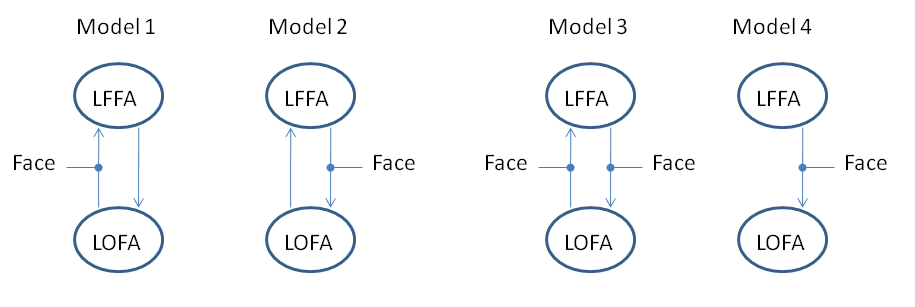
\includegraphics[width=160mm]{dcm_phase/figures/phase_models}
\caption{\em Four different DCM-Phase models  \label{dcm-phase:fig:1}}
\end{center}
\end{figure}

The connectivity for Model 4 can be set up by configuring the radio buttons as shown in Figure~\ref{dcm-phase:fig:2}. You can now press the \texttt{Invert DCM} button. It can take up to an hour to estimate the model parameters depending on the speed of your computer.

\begin{figure}
\begin{center}
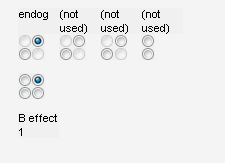
\includegraphics[width=50mm]{dcm_phase/figures/model4_conn}
\caption{\em Radio button configurations for DCM-Phase model 4  \label{dcm-phase:fig:2}}
\end{center}
\end{figure}

\section{Results}

After estimation is finished, you can assess the results by choosing from the pull-down menu at the bottom (middle). The \texttt{Sin(Data)-Region i} option will show the sin of the phase data in region $i$, for the first 16 trials. The blue line corresponds to the data and the red to the DCM-Phase model fit. The 
\texttt{Coupling(As)} and \texttt{Coupling(Bs)} buttons display the estimated endogenous and modulatory activity shown in Figure~\ref{dcm-phase:fig:3}.

\begin{figure}
\begin{center}
%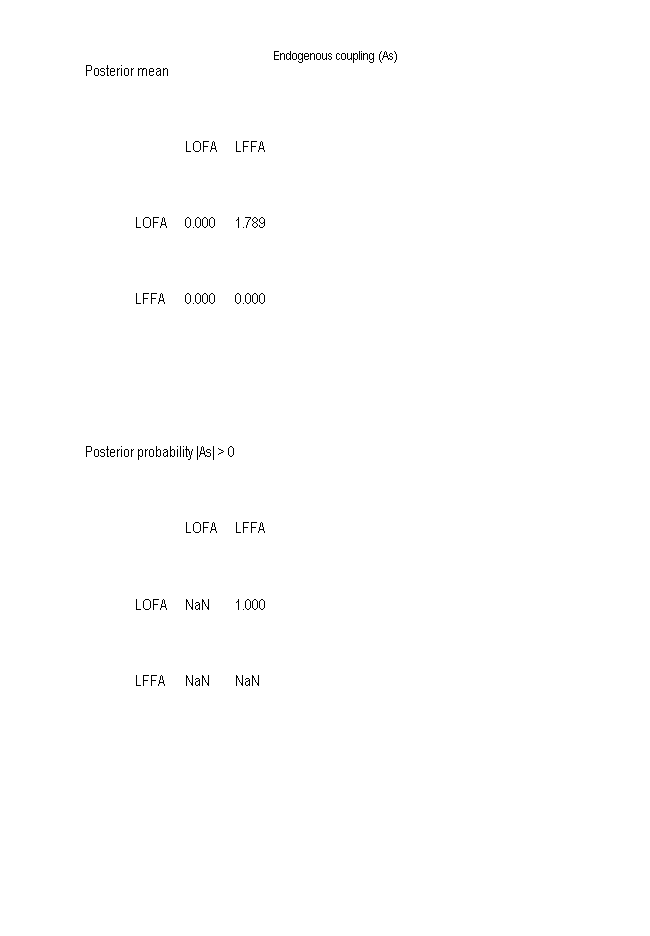
\includegraphics[width=50mm]{dcm_phase/figures/endogenous}
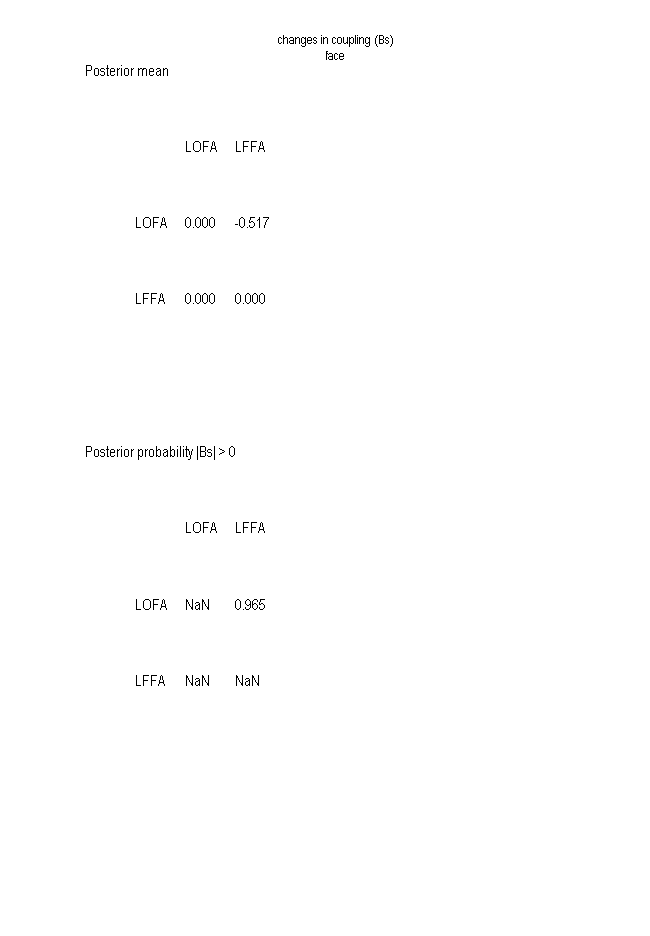
\includegraphics[width=50mm]{dcm_phase/figures/modulatory}
\caption{\em The figure shows the estimated parameters for endogenous coupling (left column) and modulatory parameters (right column) for the 4th DCM.  \label{dcm-phase:fig:3}}
\end{center}
\end{figure}

If one fits all the four models shown in Figure~\ref{dcm-phase:fig:1} then they can be formally compared using Bayesian Model Selection. This is implemented by pressing the \texttt{BMS} button. You will need to first create a directory for the results to go in e.g. \texttt{BMS-results}. For 'Inference Method' select FFX (the RFX option is only viable if you have models from a group of subjects). Under 'Data', Select 'New Subject' and under 'Subject' select 'New Session'. Then under 'Models' select the \texttt{DCM.mat} files you have created.  Then press the green play button. This will produce the results plot shown in Figure~\ref{dcm-phase:fig:4}. This leads us to conclude that 
LFFA and LOFA act in master slave arrangement with LFFA as the master.

\begin{figure}
\begin{center}
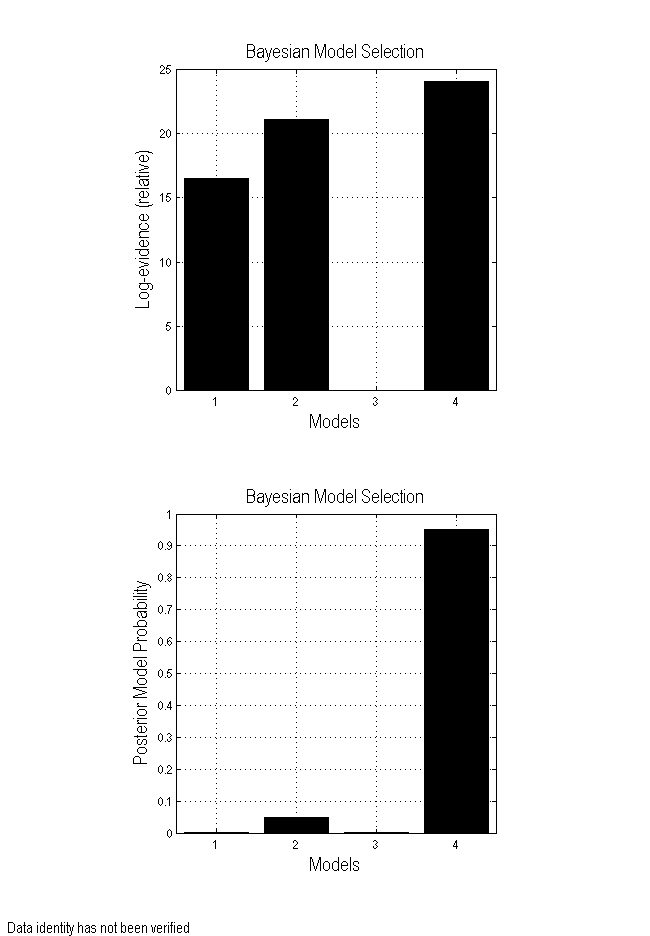
\includegraphics[width=50mm]{dcm_phase/figures/bms_phase}
\caption{\em Bayesian comparison of the four DCM-Phase models shown in Figure~\ref{dcm-phase:fig:1}.\label{dcm-phase:fig:4}}
\end{center}
\end{figure}

\section{Extensions}

In the DCM-Phase model accessible from the GUI, it is assumed that the phase interaction functions are of simple sinusoidal form ie. $a_{ij} \sin(\phi_j - \phi_i)$. The coefficients $a_{ij}$ are the values shown in the endogenous 
parameter matrices in eg. Figure~\ref{dcm-phase:fig:3}. These can then be changed by an amount $b_{ij}$ as shown in the modulatory parameter matrices. 
It is also possible to specify and estimate DCM-Phase models using matlab scripts. In this case it is possible to specify more generic phase interaction functions, such as arbitrary order Fourier series. Examples are given in \cite{dcm_phase}.
